\documentclass[10pt,a4paper]{article}
\usepackage[utf8]{inputenc}
\usepackage[francais]{babel}
\usepackage[T1]{fontenc}
\usepackage[left=2cm,right=2cm,top=2cm,bottom=2cm]{geometry}
\usepackage{graphicx}
\usepackage{moreverb}
\author{H4311}
\title{Document de Conception}

\begin{document}

\maketitle
\tableofcontents

\section{Introduction}
\subsection{Rappel du contexte}
Ce projet 4IF consiste en la conception et la réalisation d'un processeur XML comprenant les fonctionnalités suivantes : analyse syntaxique d'une DTD, analyse syntaxique d'un XML, analyse syntaxique d'un XSL, vérifications sémantiques d'un XML par rapport à une DTD donnée, transformation d'un XML par rapport à une feuille XSLT.

\subsection{Portée de ce document}
Ce document de conception présente les diagrammes de classes utilisés pour stocker en mémoire une arborescence XML et une feuille DTD, ainsi que les algorithmes de validation et de transformation.

\section{Modélisation}
\subsection{Feuille DTD}
Le schéma ci-dessous présente notre diagramme de classes au format UML pour le stockage d'une feuille DTD. Les méthodes n'ont pas été ajoutées afin de ne pas alourdir le diagramme et à la demande des enseignants.
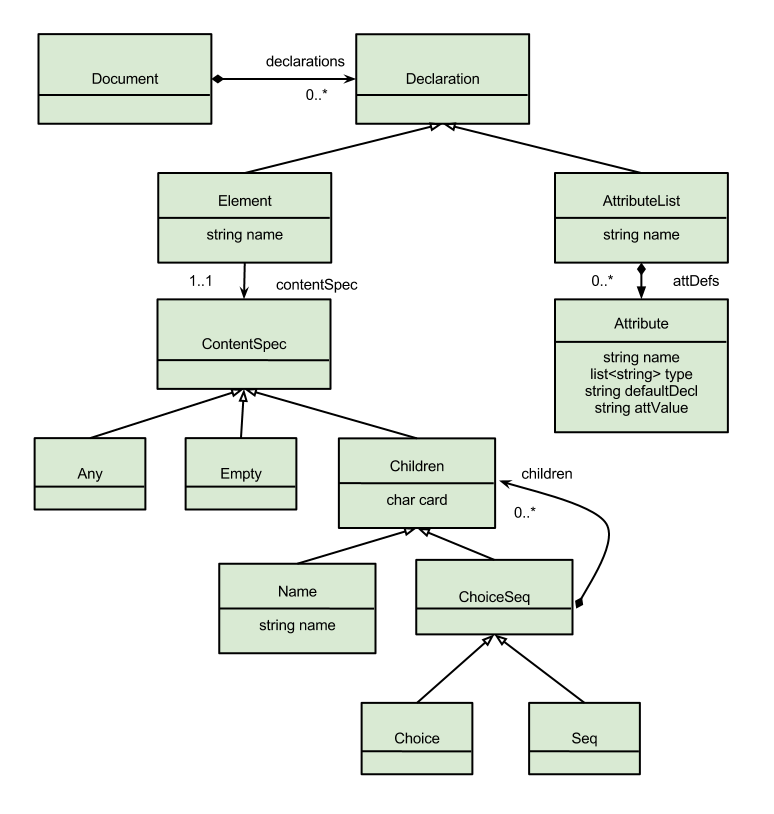
\includegraphics[scale=0.65]{DiagrammedeclasseDTD.png} 

\subsection{Document XML}
Le schéma ci-dessous présente notre diagramme de classes au format UML pour le stockage d'un document XML. Les méthodes n'ont pas été ajoutées afin de ne pas alourdir le diagramme et à la demande des enseignants.
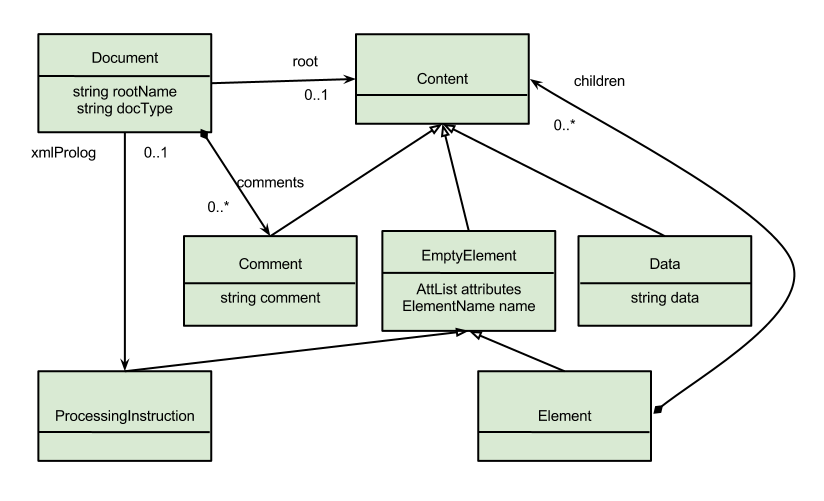
\includegraphics[scale=0.65]{DiagrammedeclasseXML.png} 

\section{Algorithmes}
\subsection{Validation}
Cet algorithme consiste en la validation d'un document XML par rapport à une DTD donnée, i.e en sa vérification sémantique.

\begin{description}
\item[Entrée :] un document XML bien formé et une feuille DTD bien formée.
\item[Sortie :] vrai si le document XML est conforme à la feuille, faux sinon.

En outre, des messages d'erreurs s'affichent sur la sortie d'erreur standard, permettant de diagnostiquer l'origine de l'erreur.
\end{description}

\paragraph{L'idée derrière l'algorithme :}
Nous partons d'un constat simple : les déclarations de contenus DTD ressemblent fortement à des expressions régulières (regex). Le principe de l'algorithme est donc le suivant :
\begin{itemize}
\item Pour chaque contenu XML, générer la chaine correspondant à ce que ce contenu a pour noeuds fils.
\item Pour chaque règle DTD, générer la regexp correspondant à cette règle.
\item Comparer la chaîne de contenu avec la règle DTD correspondante au nom de l'attribut.
\end{itemize}

\paragraph{Regex créées par les éléments dtd}
Ces fonctions servent à créer les regex des différents éléments dtd qui servent à la validation par la suite. Tous les enfants de dtd::Children dans la hiérarchie de classes dtd possèdent une version différente. Les deux premières méthodes ne prennent pas d'arguments et renvoient une chaîne correspondant à la regex générée. Les deux dernières méthodes renseignent la méthode template dtd:ChoiceSeq:regex.

\begin{itemize}
\item[dtd:Name:regex] :
\begin{verbatimtab}
	chaine regex := "(" + name + ",)"
	Si card est défini, alors
		regex += card
	FinSi
	Renvoyer regex
\end{verbatimtab}
\item[dtd:ChoiceSeq:regex] :
\begin{verbatimtab}
	caractère regexSep = getRegexSep()
	chaine regex := "("
	regex += children.premierElement.regex
	Pour tous les autres éléments c de la liste children,
		Si regexSep est non nul, alors
			regex += regexSep
		FinSi
		regex += c.regex
	FinPour
	regex += ")"
	Si card est non nul, alors
		regex += card
	FinSi
	retourner regex
\end{verbatimtab}
\item[dtd:Choice:getRegexSep] :
\begin{verbatim}
	retourner '|'
\end{verbatim}
\item[dtd:Seq:getRegexSep] :
\begin{verbatim}
	retourner vide
\end{verbatim}
\end{itemize}

\paragraph{Validation d'un élément}
\begin{description}
\item[Spécification :] Valide un noeud de l’arbre XML conformément à la DTD.
\item[Paramètres :]
\begin{itemize}
\item[content] : contenu correspondant au noeud courant.
\item[elements] : liste des éléments définis par la dtd.
\item[attributeList] : liste de liste d’attributs définis par la dtd
\end{itemize}
\item[Retour :] vrai si le noeud a été correctement validé, faux sinon.
\end{description}

\begin{verbatimtab}
validationNode(Content content, liste Element elements, list AttributeList attributeList) : booléen
Début
Si elem := content, est de type Element alors
	chaine nomBalise := elem.nom
	// Valider les attributs
	// On récupère la liste des attributs de la dtd
	Pour chaque liste d'attributs listeAtt de attributeList, faire
		Si listeAtt.nom == nomBalise, alors
			sortir de la boucle
		FinSi
	FinPour	
	Si on est sortis de la boucle manuellement,
		attributs := listeAtt.attributs
	FinSi
	// On parcourt la liste des attributs xml pour les valider
	attributsElem := elem.attributsListe
	Si taille(attributsElem) > 0, alors
		Pour tous les xml de attributsElem, faire
			booléen trouvé := faux
			Pour tous les attributs att de attributs, faire
				Si xml == att, alors
					trouvé := vrai
					sortir de la boucle
				FinSi
			FinPour
			Si trouvé == faux, alors
				Erreur := "Attribut non trouvé"
				Renvoyer FAUX
			FinSi
		FinPour
	FinSi
		
	Chaine regex = chaine vide
	Pour tous les éléments e de elements, faire
		Si e.nom == nomBalise, alors
			regex = e.nom
		FinSi
	FinPour
		
	Si regex est vide, alors
		Renvoyer faux
	FinSi
		
	children := elem.enfants
	Chaine chaineChildren = chaine vide
	Pour chaque c de children, faire
		Si c est de type Element ou EmptyElement, alors
			chaineChildren += c.nom + ','
		Sinon
			Si c est de type Data, alors
				chaineChildren += "#PCDATA,"
			FinSi
		FinSi
	FinPour

	Si la chaîne chaineChildren ne valide pas l'expression régulière regex, alors
		Renvoyer faux
    	Sinon
    		Pour chaque c de children, faire
    			resultat := Appeler récursivement validationNode(c, elements, attributesList)
    			Si resultat est faux,
    				Renvoyer faux
    			FinSi
    		FinPour
    	FinSi
    	
    	Renvoyer vrai
Fin
\end{verbatimtab}

\paragraph{Validation du document}
\begin{description}
\item[Spécification :] Valide un arbre XML par rapport à une structure de DTD.
\item[Paramètres :]
\begin{itemize}
\item[dtd] : feuille DTD.
\item[xml] : document XML.
\end{itemize}
\item[Retour :] vrai si le document a été correctement validé, faux sinon.
\end{description}

\begin{verbatimtab}
validationDocument(dtd::Document dtd, xml::Document xml) : booléen
Début
	Liste<dtd::Element> elements
	Liste<AttributesList> attributesList   
	Liste<Declarations> declarations := dtd.declarations
	
	Pour tous les d de declarations faire
		Si d est de type dtd::Element, alors
			Ajouter d à la suite de elements
		Sinon
       		Si d est de type dtd::AttributeList, alors
       			Ajouter att à la suite de attributesList
			Sinon
       			Erreur := "Une déclaration de la DTD n'est ni un dtd::Element ni un dtd::Attribute"
		FinSi
	FinPour
   
	Retourner validationNode(xml.elementRacine, elements, attributesList);
Fin
\end{verbatimtab}

\subsection{Analyse et validation XSL}
Le schéma ci-dessous résume le fonctionnement de l'algorithme :
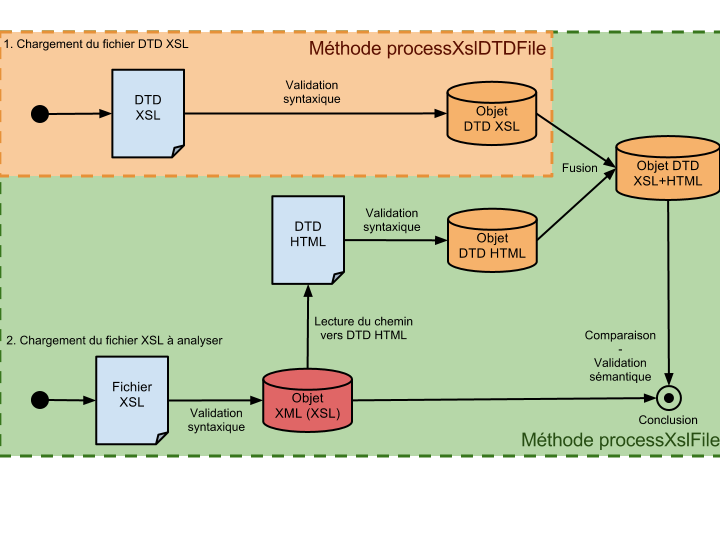
\includegraphics[scale=0.65]{Algorithmes.png} 

\subsection{Génération XSL}


\end{document}